\newcommand\tab[1][0,4cm]{\hspace*{#1}}
\newcommand\longtab[1][1cm]{\hspace*{#1}}

\chapter{Généralités}
\section{Introduction au sujet}

\paragraph*{}
Ces dernières années, la communauté des lecteurs algériens a connu une croissance rapide et le taux de participation aux salons du livre est prometteur. Avec cette quantité de livres achetés, de nouveaux problèmes voient le jour, en plus des problèmes déjà existants tels que: les prix relativement élevés de certains livres, la rareté de certains autres et la tâche difficile que les lecteurs doivent endurer pour s'identifier avec d'autres membres qui partage les mêmes intérêts et la même zone géographique, se pose le problème de stockage de ces livres et du fait qu’ils peuvent être lu par un nouveau lecteur que de prendre de la place sur une étagère quelque part.


\paragraph*{}
Il existe des clubs de lecture et des réunions sociales où les gens échangent, vendent, donnent des livres et même rencontrent de nouvelles personnes, ce qui laisse penser qu'il existe un groupe de personnes qui:

\begin{list}{•}{}
	\item Ont des livres.
	\item Sont disposés à abandonner les livres déjà lus.
	\item Veulent économiser de l’argent tout en lisent de nouveau livres
\end{list}

\paragraph*{}
Comme nous venons de le dire, certaines solutions existent pour cette communauté et nous en explorerons certaines dans les sections suivantes tout en soulignant leurs lacunes et en expliquant comment une fenêtre d'opportunités est encore ouverte pour résoudre le problème dans ces différentes aspects.

\section{Solutions déjà existants}

\subsection{Non technologiques}

\paragraph*{}
L'analyse de cette question donnera lieu à deux concepts intéressants qui existent déjà et qui sont, dans une certaine mesure, fonctionnels:

\subparagraph{{\large 1. Événements d'échange de livres}\medskip\\}

Certains clubs de lecture et cafés organisent des événements où les participants sont invités à apporter les livres qu'ils souhaitent transmettre aux autres lecteurs et à en obtenir de nouveaux dans une atmosphère conviviale.

\subparagraph*{}
\begin{list}{•}{\textbf{Avantages}}
	\item Les participants peuvent vivre toute l'expérience humaine d'échanger un livre.
	\item Les participants découvrent de nouveaux livres par des personnes autres que des simple avis en ligne.
	\item Les participants établissent des liens significatifs avec leurs collègues lecteurs de livres.
\end{list}

\subparagraph*{}
\begin{list}{•}{\textbf{Inconvénients}}
	\item De tels événements durent au mieux 2 jours, ce qui fait que beaucoup de gens ratent l'occasion.
	\item En raison de la limitation géographique, de tels événements ne peuvent être accessibles que par quelques résidents proches de la région.
	\item coûteux en terme de temps investi.
\end{list}

\newpage

\subparagraph{{\large 2. Échanges informels de livres}\medskip\\}

Certains échanges de livres sont informels - une étagère ou une boîte est fournie où les livres peuvent être laissés ou ramassés. L'échange repose sur les utilisateurs qui sortent et prennent des livres et n'est généralement pas supervisé.\medskip

C'est une pratique courante dans les auberges de jeunesse où les voyageurs peuvent laisser un livre et emporter un livre différent avec eux. Certaines gares ferroviaires en Grande-Bretagne ont des échanges de livres informels et une a également été installée dans une cabine téléphonique à Kington Magna\cite{noauthor_book_2019}.

\subparagraph*{}
\begin{list}{•}{\textbf{Avantages}}
	\item Le processus est très rapide et pratiquement pas de temps perdu.
	\item Absence de limite de temps, ils peuvent être échangés à tout moment.
\end{list}

\subparagraph*{}
\begin{list}{•}{\textbf{Inconvénients}}
	\item Le besoin de donateurs au début du projet.
	\item L'absence d'un système de contrôle de qualité pour les livres mis contre les prises.
\end{list}

\begin{figure}[h]
	\begin{center}
		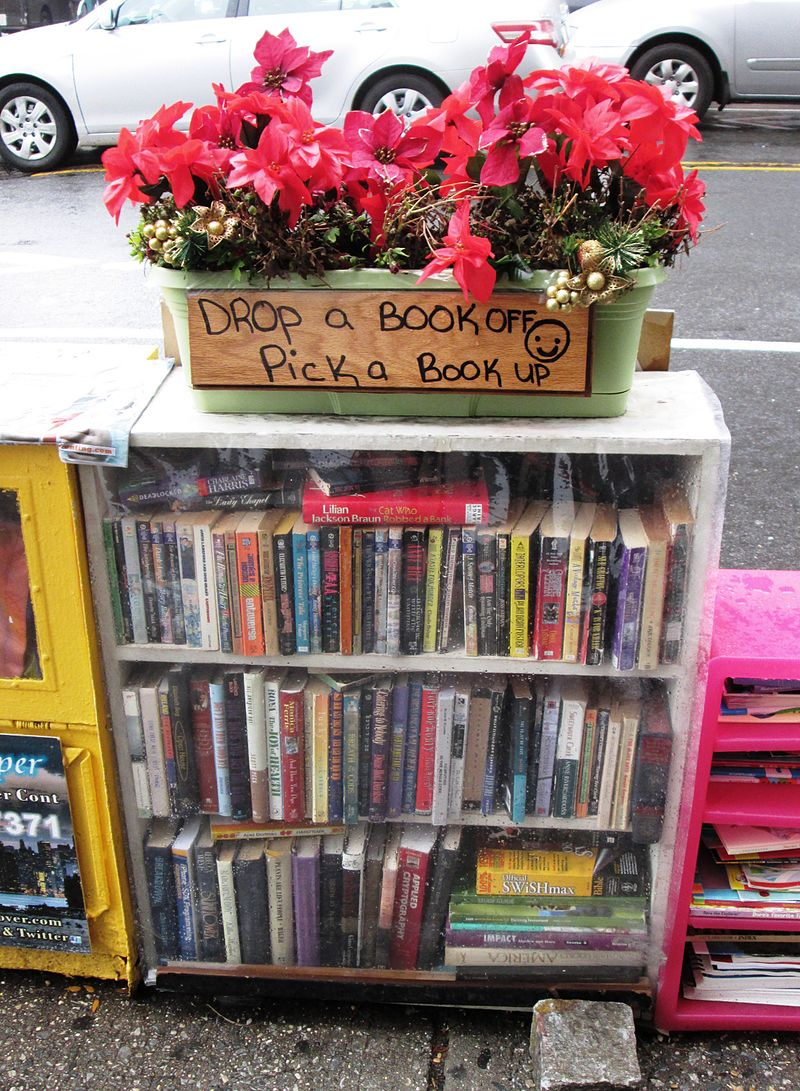
\includegraphics[width=5cm]{Images/chapter1/bookswapSpot.jpg}
		\caption{{\footnotesize Un "échange de livres de rue" à Washington Heights, New York\cite{noauthor_book_2019}}}
	\end{center}
\end{figure}

\newpage

\subsection{Technologiques}

\paragraph*{}
Il existe plusieurs sites Web et très peu d'applications populaires offrant le type de bonne expérience présente dans la manière traditionnelle, nous allons explorer certaines des plus populaires solutions existant aujourd’hui.\\

\subparagraph{{\large 1. BookMooch}\medskip \\}

\begin{wrapfigure}[13]{r}{3.5cm}
	\raisebox{0pt}[\dimexpr\height+1.5\baselineskip\relax]{
\includegraphics[width=3.5cm]{Images/chapter1/bookMoochLogo.jpg}}
	\caption{{\footnotesize Logo de BookMooch}}
\end{wrapfigure}

Portant bien son nom, avec le fameux slogan \textit{​“Give books away, Get books you want”},BookMooch est une société de publication delivres en ligne par laquelle ses membres peuvent échanger des livres entre eux. Son fondateur,
John Buckman, a choisi ce nom pour l'entreprise en référence à l'acte de donner un livre sans attendre de le récupérer. Les utilisateurs, alors, sont considérés comme des BookMoochers et bénéficient à bien des égards de ce système commercial unique.

En bref, les utilisateurs «achètent» les livres des autres membres	en utilisant uniquement des points. Chaque membre peut accumuler des points en soumettant les titres des livres qu'il veut donner et en envoyant ses livres à d'autres utilisateurs. Avec suffisamment de points, ils peuvent alors commencer à recevoir les titres d'autres personnes, et le processus continue à partir de là. Le seul coût pour les membres est celui de l'envoi des livres qu'ils envoient à d'autres.\cite{noauthor_bookmooch_nodate}\\

\subparagraph*{}
\begin{list}{•}{\textbf{Avantages}}
	\item L'adhésion à cette entreprise est gratuite.
	\item Vous pouvez choisir parmi une grande variété de livres.
	\item Une liste de souhaits connectée à amazon où vous recevrez des notifications lorsque des livres sont disponibles.
\end{list}

\subparagraph*{}
\begin{list}{•}{\textbf{Inconvénients}}
	\item Pour recevoir, il faut donner.
	\item Dans une certaine mesure, la plate-forme peut être un terrain de jeu pour les fraudeurs.
	\item La plate-forme n'exploite pas l'emplacement des membres.
\end{list}

\subparagraph{{\large 2. Bookup}\medskip \\}

\begin{wrapfigure}[8]{r}{2.5cm}
		\raisebox{0pt}[\dimexpr\height+2\baselineskip\relax]{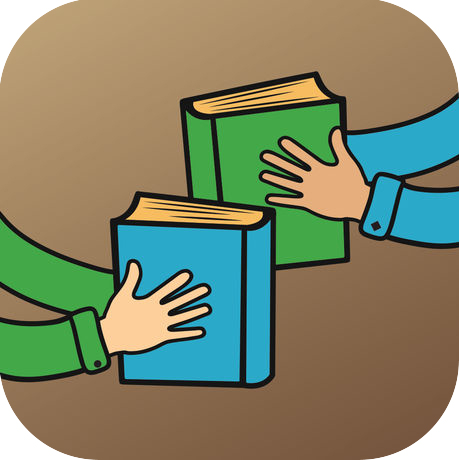
\includegraphics[width=2.5cm]{Images/chapter1/bookUpLogo.jpg}}
		\caption{{\footnotesize Logo de Bookup}}
\end{wrapfigure}

L'application Bookup est destinée aux lecteurs de livres imprimés qui souhaitent échanger leurs livres contre d'autres livres de leur région, gratuitement, et éventuellement se faire un nouvel ami partageant le même intérêt pour la lecture. Bookup fournit une fonctionnalité d’échange de livre en fonction de l’emplacement.\cite{noauthor_bookup_nodate-1}\\

\subparagraph*{}
\begin{list}{•}{\textbf{Avantages}}
	\item La plate-forme exploite l'emplacement des membres.
	\item Fonctionnalité de bibliothèque personnelle que vous pouvez personnaliser à votre guise.
	\item Liberté absolue pour les utilisateurs de discuter en temps réel et de trouver un moyen d'exécuter l'échange.
	\item Un mécanisme simple d'exploration aléatoire de livres proches.
\end{list}

\subparagraph*{}
\begin{list}{•}{\textbf{Inconvénients}}
	\item L'application est disponible uniquement sur les appareils marchent avec iOS.
	\item Une expérience utilisateur moyenne.
	\item Un manque évident d'informations sur les livres et les utilisateurs.
\end{list}

\begin{figure}[h]
	\begin{center}
		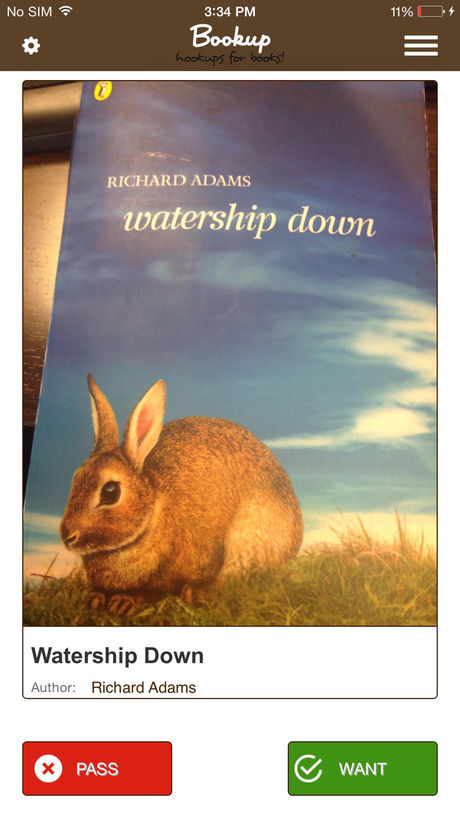
\includegraphics[width=3cm]{Images/chapter1/bookUpScreenshot.jpg}
		\caption{\footnotesize {Le mecanisme de suggestion et decouverte offert par Book Up ou l'utilisateur parcours une pile de cartes des livres près de son zone géographique on choisissent “passer” ou “vouloir”}}
	\end{center}
\end{figure}
\newpage

\subparagraph{{\large 3. Bookabikia\medskip \\}}

%raisedbox is for adding margin to wrapfigure
\begin{wrapfigure}[8]{r}{4cm}
	\raisebox{0pt}[\dimexpr\height+2.5\baselineskip\relax]{
\includegraphics[width=4cm]{Images/chapter1/bookabikiaLogo.png}}
	\caption{{\footnotesize Logo de Bookabikia}}
\end{wrapfigure}

Bookabikia est une plate-forme et un service fabriqués en Égypte qui permettent aux gens d'échanger des livres. L'équipe derrière le projet a fait un excellent travail en résolvant non seulement les problèmes évidents auxquels la communauté des lecteurs est confrontée, mais également en l'exploitant avec brio. Sur le site Bookabkia, vous ferez une demande de don pour le site avec vos livres. L’équipe de livraison viendra à vous pour prendre les livres dans les jours à venir et 24 heures après avoir reçu les livres, vous obtiendrez un crédit qui se présente sous forme de points, avec ce crédit, vous pourrez acheter plusieurs livres en même temps sans avoir besoin d’intérêt personnel pour vos livres.\cite{noauthor_bookabikia_nodate}

\subparagraph*{}
\begin{list}{•}{\textbf{Avantages}}
	\item Les utilisateurs ne sont pas obligés de passer des offres d'échange avec d'autres utilisateurs.
	\item La fonction de crédit donne beaucoup de liberté de choix aux gens.
	\item Tous les livres sont expédiés au domicile de l'utilisateur.
\end{list}

\subparagraph*{}
\begin{list}{•}{\textbf{Inconvénients}}
	\item La plate-forme ne permet pas les interactions peer-to-peer entre les membres de la communauté.
	\item Le service n'est pas totalement gratuit.
	\item L'expérience utilisateur n'est pas personnalisable.
\end{list}

\begin{figure}[h]
	\begin{center}
		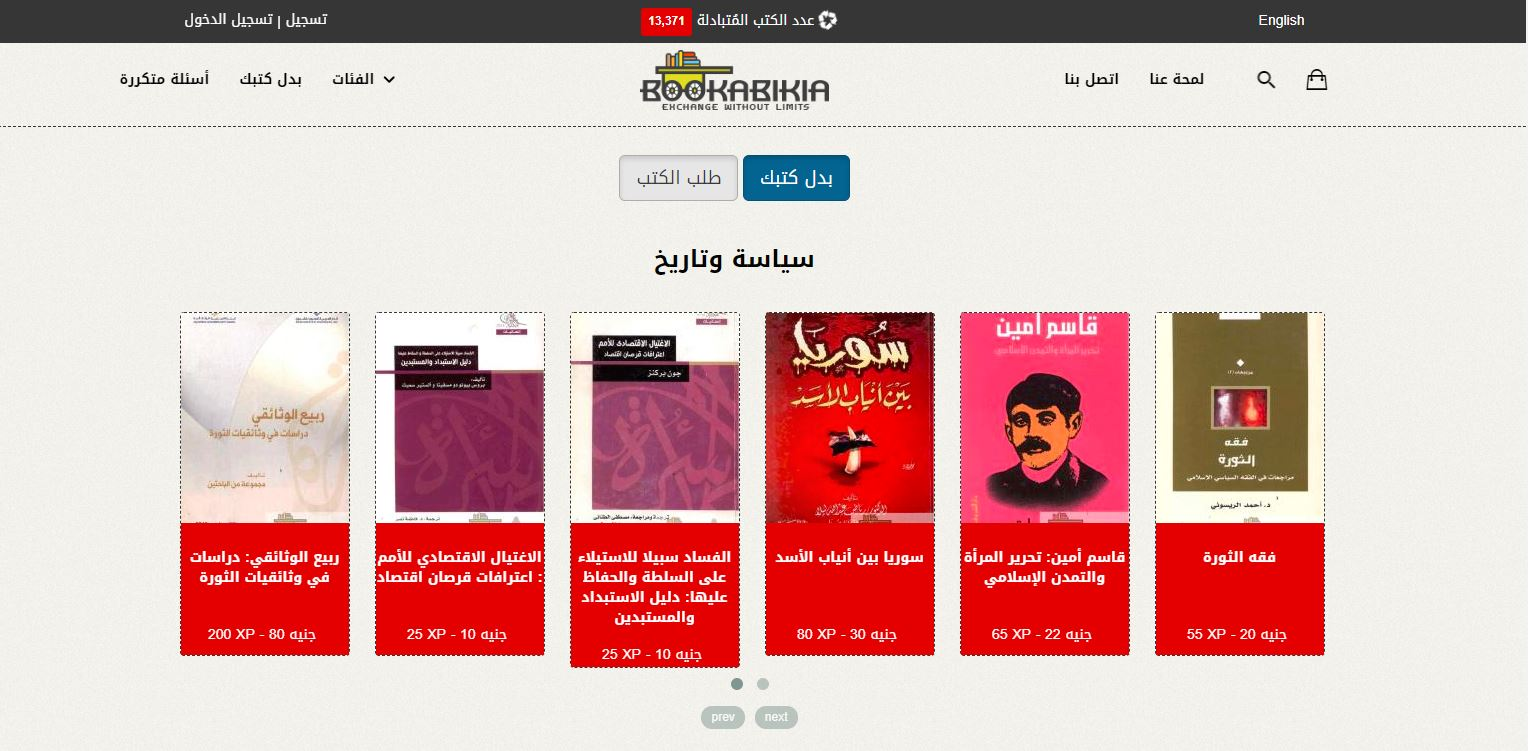
\includegraphics[width=9cm]{Images/chapter1/bookabikiaScreenshot.jpg}
		\caption{{\footnotesize Page d'acceuil de Bookabikia}}
	\end{center}
\end{figure}

\newpage
\section{Solution proposé}
\paragraph*{}
Aussi merveilleux que les solutions existantes sont, nous pensons pouvoir encore offrir une meilleure solution et une meilleure expérience, en exploitant deux aspects de la pratique de l'échange de livres:

\begin{list}{•}{}
	\item La sociabilité humaine et la capacité à s'identifier aux autres et à créer de petites communautés et des relations durables et significatives.
	\item Une interface utilisateur magnifique et une expérience utilisateur personnalisable qui permettent une totale liberté d'interaction avec d'autres utilisateurs.
\end{list}

La solution consiste en une application mobile fonctionnant à la fois sur Android et sur iOS (97,43\% des appareils du monde (Android et iOS) \cite{noauthor_mobile_nodate}), où les utilisateurs enregistrés peuvent:

\begin{list}{•}{}
	\item Créez un profil et répertoriez tous les livres qu’ils possèdent et sont disposés à échanger, prêter, vendre ou même faire un don à un autre utilisateur de leur choix. Le tout dans une interface utilisateur magnifiquement structuré.
	\item Recherchez les livres qu'ils souhaitent acquérir en utilisant des mécanismes de recherche avancés qui permettent d'obtenir les résultats les plus homogènes, les plus fonctionnels et les plus pratiques.
	\item Explorez les utilisateurs à proximité (propriétaires de livres) a l'aide de la map, parcourez leurs bibliothèques d'un simple balayage et d'un clic.
	\item Envoyez et recevez des messages en temps réel avec le service de messagerie, sans aucune limitation.
\end{list}

Enfin, l’application portera le nom «Bindex», qui est une forme abrégée d’index de livre qui résume le travail que l’application accomplit en indexant toutes les bibliothèques personnelles et en les mettant au bout du doigt d’un utilisateur donné.

\begin{figure}[h]
	\begin{center}
		\raisebox{0pt}[\dimexpr\height+2\baselineskip\relax]{
\includegraphics[width=6.5cm]{Images/chapter1/bindexLogo.png}}
		\caption{{\footnotesize Logo de Bindex}}
	\end{center}
\end{figure}

\section{Plan du rapport}
\paragraph*{}
Après avoir passé en revue les généralités et l’introduction, nous plongerons dans la manière dont ce projet prospère va prendre vie:
\paragraph*{}
Dans le deuxième chapitre, nous aborderons les technologies et les solutions les plus appropriées pour la réalisation de l’application mobile, en mentionnant également certains services de base utilisés, et dans le chapitre suivant, nous aborderons les processus qui ont été pris en compte pour la création. de l’application, de la conception initiale et brouillon au prototypage et aussi le développement, tout en soulignant les outils utilisés, ainsi que les mécanismes de co-travail et les outils qui ont permis de faire de l’ensemble du projet une expérience fluide.
\paragraph*{}
Après cela, nous plongerons encore plus profondément dans une démonstration où nous présenterons toutes les fonctionnalités qui ont été développées et comment nous prévoyons de nous développer à l’avenir.

